% (c) GreenSocs Ltd
% author: Christian Schroeder <schroeder@eis.cs.tu-bs.de>

\cleardoublepage
\chapter{Introduction}

The \GreenConfig project aims to provide a library that can be used to connect User defined configuration mechanisms to Tool configuration mechanisms, giving both flexibility. 

The diagram \ref{fig:config} shows an IP block connected, via the configuration library, to an ESL tool that is providing configuration from a database. 

The IP block has one API to the library. The library uses a different API to the ESL tool. 

\begin{figure}[htbp]
	\centerline{
		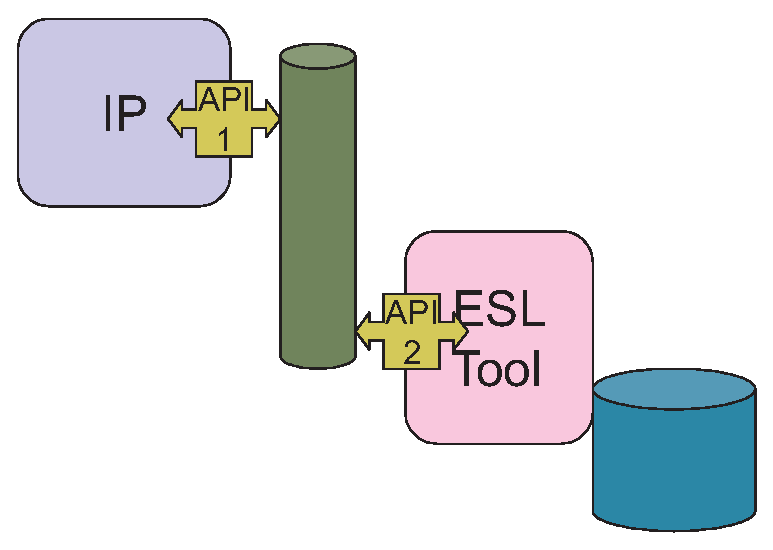
\includegraphics[width=10cm]{config.eps}} 
	\caption{IP block, ESL tool and GreenConfig Library}
	\label{fig:config}
\end{figure}

This allows IP designers to choose the configuration mechanism that best suits their style of IP creation, while staying independent of tools.  

\section{GreenControl Middleware}
See the \hypertarget{GCUsersGuide}{\href{http://www.greensocs.com/projects/GreenControl/docs/GCUsersGuide}{\GreenControl User's Guide}} and web page\footnote{\GreenControl project page:  \href{http://www.greensocs.com/projects/GreenControl}{http://www.greensocs.com/projects/GreenControl}} for a description of the \GreenControl framework which is the base of \GreenConfig.

\subsection{User APIs}

\paragraph{Config APIs}
Config APIs are \emph{special \GreenControl User APIs} whose task is the parameter configuration (\GreenConfig) and communicate with the \emph{ConfigPlugin}. 

\begin{itemize}
	\item Different API calls are translated into transactions with different command fields performing the actions inside the plugin.
	\item Config APIs receive transactions from the ConfigPlugin and process them, e.g. notification of value change events.
\end{itemize}

Config API implementations should be kept minimalistic. Each parameter access leads to a transaction to the ConfigPlugin. The other way around the developer of an API may want to cache parameter values locally.

There are different types of configuration User APIs:
\begin{itemize}
	\item GreenConfig parameters (gs\_param) are the default native objects that should be used to make a model configurable.
	\item The GreenConfig API (GCnf\_Api) is the native API to be used by any configurating unit (e.g. testbenches, tools, models configuring other models)
	\item Several adapter APIs allow integration of other configuration mechanisms or models using those.
\end{itemize}


\section{ConfigPlugin}
The ConfigPlugin is a GreenControl Service Plugin. It provides all functionality required by the Config APIs (cp. requirement list in appendix \ref{requirements}).


\section{Parameter management}
The configurable parameters are managed by the ConfigPlugin. To load and store parameters, it uses a Param-API which is connected to a storage implementation. This might be  

\begin{itemize}
	\item a simple map  
	\item an SQL database 
	\item ... 
\end{itemize}
